%Title Data
\documentclass[reqno]{amsart}
\title{Literature Review \& Project Outline}
\author{Fergus Barratt}
\date{\today}
\thanks{First Supervisor: Marzena Szymanska \\Second Supervisor: Themis Mavrogordatos}
%Packages
\usepackage{amsmath}
\usepackage{mathrsfs}
\usepackage[margin=0.7in]{geometry}
% \usepackage{fullpage}
\usepackage{graphicx}
\usepackage[backend=biber, style=ieee]{biblatex}
\usepackage{todonotes}
\usepackage{graphicx}
\usepackage{float}
\usepackage{caption}
\usepackage{subcaption}
\usepackage{grffile}
\usepackage{cleveref}
\graphicspath{ {./Images} }

% section hack
\makeatletter
\@addtoreset{section}{part}
\def\@part[#1]#2{%
    \ifnum \c@secnumdepth >\m@ne
          \refstepcounter{part}%
      \addcontentsline{toc}{part}{\thepart\hspace{1em}#1}%
    \else
      \addcontentsline{toc}{part}{#1}%
    \fi
    {\parindent \z@ \raggedright
     \interlinepenalty \@M
     \normalfont\centering
     \ifnum \c@secnumdepth >\m@ne
       \LARGE\bfseries \partname\nobreakspace\thepart
       \par\nobreak
     \fi
     \huge \bfseries #2%
     \markboth{}{}\par}%
    \nobreak
    \vskip 3ex
    \@afterheading}
\renewcommand\partname{Section}
\makeatother

\addbibresource{Bibliography.bib}

%Operator,math and QM shorthands
\newcommand{\ham}{\hat{\mathscr{H}}}
\newcommand{\cre}{\hat{a}^\dagger}
\newcommand{\ann}{\hat{a}}
\newcommand{\atann}{\hat{\sigma}_-}
\newcommand{\atcre}{\hat{\sigma}_+}
\newcommand{\dens}{\hat{\rho}}
\newcommand{\ket}[1]{| #1 \rangle}
\newcommand{\bra}[1]{\langle#1 |}
\newcommand{\braket}[2]{\langle#1 | #2 \rangle}
\newcommand{\bratens}[2]{\bra{#1} \otimes\bra{#2}}
\newcommand{\kettens}[2]{\ket{#1} \otimes\ket{#2}}
\newcommand{\qexp}[1]{\langle#1 \rangle}
\newcommand{\Epsilon}{\mathcal{E}}
\newcommand{\schro}[2]{i \hbar\ket{#1} = #2 \ket{#1}}

\begin{document}
\maketitle
%%!TEX root = LiteratureReview.tex
\begin{titlepage}
    \begin{center}
        \vspace*{1cm}
        
        \huge Literature Review \& Project Outline
        
        \vspace{1.5cm}
        \normalsize
        \emph{Fergus Barratt}
        
        \vfill
        \large
        First Supervisor: Marzena Szymanska\\
        Second Supervisor: Themis Mavrogordatos
        
    \end{center}
\end{titlepage}
 %-------------------------------------------------------------------------------------------------------------------------------
% \todo[inline]{Change HJC section to definition via $\Omega_n$}
% \todo[inline]{justification of Lindblad form}
% \todo[inline]{dispersive regime}
% \todo[inline]{Finish summary of Carmichael paper}
 %--------------------------------------------------------------------------------------------------------------------------------
%!TEX root = LiteratureReview.tex


\section{Project Outline}
This project investigates a phase bistability in the driven Jaynes Cummings model, and its representation in terms of quasiprobability functions. 

By performing computational simulations and analytical models we plan to investigate the Jaynes-Cummings model from this viewpoint, with particular focus on the dispersive case - i.e. when the cavity and qubit are far detuned from one another. 

\section{Timeline}
Until Christmas 2015 we will be familiarising ourselves with the driven Jaynes-Cummings model in the resonant case, starting with the paper by Carmichael that is summarised in the Literature Review. Beyond that, we plan to move to the dispersive regime, and compare results from this methodology with those produced by the other Masters student on the project who is producing Monte Carlo simulations of the same system.

% By the end of this project familiarity with the Markovian quantum master equation will be acquired along with the quasi-probability formulation of quantum optics through the positive P-representation approach. The role of the cavity as a meter will be investigated by performing Von Neumann projective measurements on the qubit observable in the strong coupling regime, through the correlation of photon pointer states and the qubit eigenstates.


\part{Literature Review}
\section{Introduction\autocite{Breuer2002}}
Consider a statistical ensemble $\varepsilon$ consisting of a suitably large number N of identically prepared quantum systems
\begin{equation}
  \varepsilon = \{S^1, S^2, \ldots, S^N\}
\end{equation}
Such a statistical ensemble represents a particular set of experimental conditions, whose realisation in each instance generates a particular member $S^i$ of  $\varepsilon$

The first postulate of the statistical interpretation of quantum mechanics is that a complete characterisation of such a statistical ensemble can be represented by a normalised state vector $| \psi \rangle$ in an associated Hilbert space $\mathcal{H}$

The second postulate is that all the possible outcomes of measurements on such an ensemble are represented by self-adjoint operators on $\mathcal{H}$. The outcome of the measurement corresponding to an operator $\hat{R}$ represents a real valued random variable R with cumulative distribution function $F_{\hat{R}}$ defined via the family of orthogonal projection operators that constitute the spectral decomposition of $\hat{R}$:
\begin{equation}
  \hat{R} = \int_{-\infty}^\infty rdE_r
\end{equation}
as
\begin{equation}
  F_{\hat{R}} = \langle \psi |E_r | \psi \rangle
\end{equation}
This characterisation of the possible statistical variation of a quantum system is not yet complete, for it neglects classical uncertainty associated with which statistical ensemble $\varepsilon$ represents a given quantum system. To generate the most general possible representation of a quantum statistical ensemble, a number of possible quantum ensembles $\varepsilon_\alpha$ of the above type are mixed with weights $w_\alpha$ (these weights are probabilities in the classical, not quantum sense). A self-adjoint operator now yields a random variable R with cumulative distribution function
\begin{equation}
  F_{\hat{R}} = \sum_\alpha w_\alpha \langle \psi_\alpha | E_r | \psi_\alpha \rangle
\end{equation}
for convenience, the \emph{density operator} $\rho$ can be introduced thus
\begin{equation}
  \dens = \sum_\alpha w_\alpha |\psi_\alpha \rangle \langle \psi_\alpha |
\end{equation}
and the cumulative distribution written:
\begin{equation}
  F_{\hat{R}} = tr\{E_r \dens \}
\end{equation}
by a similar mixing argument and using the spectral decomposition of $\hat{R}$ the mean and variance of the random variable associated with $\hat{R}$ as above are as follows
\begin{align}
  \langle \hat{R} \rangle &= tr\{\hat{R} \dens \} \\
  var(\hat{R}) &= \langle \hat{R}^2 \rangle - {\langle \hat{R} \rangle}^2
\end{align}
The density matrix constitutes a complete description of the statistical properties of an open quantum system. Thus, the dynamics of such a system can be described by the time evolution of its density operator.
%----------------------------------------------------------------------------------------------------------------------------------
%!TEX root = Thesis.tex

\section{The Quantum Master Equation}
The quantum master equation is in a sense a generalisation of the classical master equation, which describes the time evolution of a system confined to a set of states via a set of differential equations for the probability of the system occupying each state. In the quantum case, differential equations not just for the probability of occupying a particular state (the diagonal elements of $\dens$) are required, but also equations describing how the off diagonal elements of the density matrix evolve in time because of their relation to quantum coherence effects.

In the nonrelativistic theory of quantum mechanics the time evolution of the pure state state vector is described by the \emph{Schr\"odinger equation}:
\begin{equation}
	i\hbar \frac{d}{dt} |\psi(t)\rangle = \ham(t) |\psi(t) \rangle
\end{equation}
with $\ham$ the Hamiltonian of the system. Setting $\hbar$ to 1 going forwards, the time dependence in the above can also be represented in terms of a time evolution operator (generated by the Hamiltonian)
\begin{equation}
	|\psi(t) \rangle = U(t, 0) | \psi(0) \rangle
\end{equation}
by substitution of the (10) into (9), it is easy to see that $U^{\dagger}U = UU^\dagger = I$ provided $\ham$ is hermitian i.e. U represents unitary time evolution of the system

For a mixed state of a closed system, an equation of motion for the density matrix
\begin{equation}
	\dens (t) = \sum_\alpha w_{\alpha} |\psi_\alpha (t) \rangle \langle \psi_\alpha (t) |
\end{equation}
can be found by propagating each normalised $| \psi_\alpha (t) \rangle$ with the unitary time evolution operator given by solving the Schr\"odinger equation, the net result of which is more concisely expressed
\begin{equation}
	\dens (t) = U(t, 0)\dens (0) U^\dagger (t, 0)
\end{equation}
which, when differentiated with respect to time yields the \emph{Liouville-Von Neumann} equation
\begin{equation}
	\frac{d}{dt}\dens(t) = i [\ham, \dens (t) ]
\end{equation}
Non-unitary dynamics of open systems result from partitioning a larger, unitarily evolved system into system and environment, and performing a partial trace over the environment degrees of freedom.

We start with the Hamiltonian for a closed, potentially mixed, potentially time dependent quantum system and partition it into components representing: a subsystem constituting the totality of the interesting dynamics: the \emph{system}, a subsystem representing the dynamics of the remaining subsystem the \emph{environment} or \emph{reservoir}, and a component representing the interaction between system and environment (there is an associated partitioning of the Hilbert space into the tensor product of system and environment Hilbert spaces, and in the equation below it is understood that operators with the subscript S operate only on the system degrees of freedom i.e. exist in the system Hilbert space and represent identity in the environment Hilbert space, and etc.)
\begin{equation}
	\ham = \ham_S +\ham_R + \ham_I
\end{equation}
The partial trace operation is an operator-valued function that takes a operator on a larger Hilbert space and discards its action on all but a smaller Hilbert space, colloquially ``tracing over'' the degrees of freedom of the discarded subsystem to leave the operator on a smaller subsystem.

Starting from the equation for the unitary time evolution and tracing over the environment
\begin{equation}
	\dens_S (t) = tr_E \{U(t, 0) \dens_S (0) U^\dagger (t, 0) \}
\end{equation}
with $\dens_S = tr_E\{\dens \}$ we arrive at the most general form for evolution of the \emph{reduced} system, also known as the reduced master equation
\begin{equation}
	\frac{d}{dt} \rho_S (t) = -itr_E\{[\ham(t), \dens_S(t)]\}
\end{equation}
Which is presented in full generality
\subsection{Quantum Measurements}
One general theory of non unitary evolution is furnished by the generalised theory of quantum measurement \cite{Wiseman2010a}
\subsubsection{Von-Neumann projective measurements}
The standard formulations of quantum mechanics considers measurements via the Von-Neumann-L\"uders Projection Postulate\cite{Dirac1927}
\newtheorem{definition}{Definition}
\begin{definition}
    The result of a measurement of operator $A$ with spectral decomposition $A = \sum_\lambda \lambda \hat{\Pi}_\lambda $, (for $A$ with discrete, non-degenerate spectrum) is an eigenvalue $lambda$, and state of the system conditioned on receiving such a value is given by
    \begin{equation}
        \rho_\lambda = \frac{\hat{\Pi}_\lambda \rho \hat{\Pi}_\lambda}{Tr[\rho\hat{\Pi}_\lambda]}
    \end{equation}
\end{definition}
The quantum analog of the Bayesian rule for the update of probabilities.
In general, such a description does not represent the measurements that experimentalists perform on quantum systems, and nor does it consider the coupling of every real quantum system to its environment. More generally, we deal with the formalism of Operators \& Effects.

We consider a probe (or pointer/meter/apparatus) system through which we measure the system of interest. Let the initial state of the combined probe-system state be a pure product of probe-system kets
\begin{equation}
  | \Psi (t) \rangle = | \theta (t) \rangle \otimes | \psi (t) \rangle
\end{equation}
We let the coupled system evolve unitarily for some time $t_1$, entangling the system and the probe. We now perform a Von-Neumann projective measurement on the probe, through some projector $\pi_\lambda = \Pi_\lambda \otimes \hat{I}$ acting only on the probe space over some second period of time $t_2$ with $t_1 + t_2 = T$. From the projection postulate, we have as conditional final state:
\begin{equation}
    | \Psi_\lambda (t+T) \rangle = \frac{\pi_\lambda U(t_1) |\Psi(t)\rangle}{P}
\end{equation}
where P is the probability that we obtain result $\lambda$ when measuring the probe.

Measuring the entangled state projectively disentangles the probe and the system and represents an operation on the system space given by
\begin{equation}
\Psi_\lambda = | \lambda \rangle \hat{M}_\lambda | \psi(t) \rangle / P
\end{equation}
 where we implicitly consider nondegenerate spectra by decomposing the projector $\Pi_\lambda = |\lambda \rangle \langle \lambda |$, and where
 \begin{equation}
     \hat{M}_\lambda = \langle \lambda | U(t_1) | \theta(t) \rangle
 \end{equation}
 is the \emph{measurement operator}, which now acts only only on the system Hilbert space. The normalisation factor P is expressed in terms of these operators
 \begin{equation}
     P^2 = \langle \Psi (t) | \hat{M}_\lambda^\dagger \hat{M}_\lambda | \Psi (t) \rangle
 \end{equation}

 Our description of the measurement process has been so far effectively independendent of the meter. We can thus abstract over the particular form of the probe state. The state of the system following the generalised measurement process is given through the measurement operators $\hat{M}_\lambda$ as follows
 \begin{equation}
 | \psi_\lambda (t + T) \rangle = \hat{M}_\lambda | \psi(t) \rangle /P
 \end{equation}
 and the probability that the system takes some state is given through the \emph{effects} (probability operators) $ \mathscr{E}_\lambda = \hat{M}_\lambda^\dagger \hat{M}_\lambda $ as
 \begin{equation}
     P^2 = \mathscr{P}_\lambda = \langle \psi_\lambda (t) | \mathscr{E}_\lambda | \psi_\lambda \rangle
 \end{equation}
 the set $\{\mathscr{E}_\lambda | \sum_\lambda \mathscr{E}_\lambda = \hat{I} \} $ is known as a POVM: a \emph{Positive Operator Valued Measure} \footnote{Positivity is clear since the operators $\hat{M}_\lambda$ are positive. Positivity, and that the operators resolve unity constitute the only restrictions on these operators}

 We now consider a finite sequence of quantum measurements of this kind. From the above, after some given timestep T, (we now consider propagating mixed states rather than pure states)
 \begin{equation}
     \rho_\lambda (T) = \mathscr{F}[\hat{M}_\lambda] \rho(0) / \mathscr{P}_\lambda
 \end{equation}
 With $\mathscr{F}[\hat{M}_\lambda] ( \hat{O} ) =  \hat{M}_\lambda \hat{O} \hat{M}_\lambda ^ \dagger$ a \emph{superoperator}
 This superoperator is an \emph{operation} for the value $\lambda$. We consider the superoperators that represent physical time evolution.
 \subsubsection{Physical Dynamical Maps}
A dynamical map is a map that takes a dynamical system at a time t to the same system at a time t'. In considering such a map on density matrices $\Phi$, we require that it meet certain criteria
\begin{enumerate}
    \item \emph{Linearity}. We require that moving a system forwards in time respects the tensor product structure of quantum mechanics
        \begin{equation}
            \Phi_T[\alpha\rho(t) + \beta\rho'(t')] = \alpha \Phi_T[\rho(t) + \beta \Phi_T[\rho'(t')]
        \end{equation}
    \item \emph{Complete Positivity}. We require that density matrices remain positive for all time. More strictly, we require that the operation of propagating some subsystem leaves the density matrix of the supersystem positive.
        \begin{align}
            p & \in  spectrum \{\Phi_T[\rho(t)]\} \geq  0\quad \forall p, T, t\\
            p & \in  spectrum \{\Phi_T \otimes \hat{I} [\rho_A(t) \otimes\rho_B(t) ] \} \geq 0 \quad \forall p, T, t
        \end{align}
        where the second inequality is true for all possible partitionings of the system into subsystems.
    \item \emph{Trace-Preserving}. We require that the trace of the density matrix is invariant under time propagation
        \begin{equation}
            tr\{ \Phi_T[\rho_t] \} = tr \{ \rho_t \} \quad \forall t, T
        \end{equation}
\end{enumerate}
It is a fundamental theorem of Kraus \cite{Kraus1983} that any such superoperator can be represented\cite{Nielsen2010}
\begin{equation}
    \Phi[\rho] = \sum_k \mathscr{E}_k^\dagger \rho \mathscr{E}_k
\end{equation}
where $\mathscr{E}_k $ are known as Kraus Operators, but are exactly the measurement operators $\mathscr{E}_\lambda$ derived above. This decomposition is known as the Operator-Sum representation\cite{Nielsen2010}, and operators satisfying the above conditions are CPTP (Completely Positive, Trace-Preserving) maps. The problem of describing the time evolution of a density operator reduces to finding the Kraus operators that represent the superoperator that generates the system time evolution.

This process admits a clear interpretation. The nonunitary time evolution of a system corresponds to a countable series of measurement steps, where the system is non-orthogonally projected at each time step by the POVM consisting of the Kraus operators that give its time evolution.
\subsection{Quantum Dynamical Semigroups}
Markovian processes are colloquially ``memoryless'', a classical example being Brownian Motion. Whilst the operator-sum representation can represent a more general time-evolution, most analytically solvable situations invoke what is known as the markov approximation. Here we derive the master equation in the Markov approximation via the theory of Dynamical Semigroups, and in a microscopic formulation
\subsubsection{Markov Processes}
Classical Markov processes are characterised by the invocation of the so-called semigroup property of the Chapman-Kolmogorov equation. The Markov transition probabilities $T(x, t|x', t')$ form a one parameter semigroup in t, because of the composition property $T(x, t|x, t')T(x, t'|x, t``) = T(x, t|,x, t``)$ which results from the conditions that memorylessness puts on their form. This memorylessness is also responsible for this being a \emph{semi}group, since there does not in general exist an inverse for each element-there exist irreversible Markov processes.
This semigroup is in fact a "contracting" semigroup, in that the norm of a propagated probability is less than or equal to the probability.
The generalisation of Markov processes to quantum mechanics analagously leads to the theory of \emph{quantum dynamical semigroups}

\subsubsection{Lindblad Form}
The most general form\cite[119--122]{Breuer2002} for the reduced master equation in the Markov approximation is known as the \emph{Lindblad Form}
\begin{align}
        \frac{d}{dt} \rho_S (t) =& -i[\ham (t), \dens (t)\notag]\\
                                 & + \sum_{k=1}^{N^2-1} \gamma_k \{ \hat{A}_k \dens_S \hat{A}_k -\frac{1}{2}  \hat{A}_k \dens_S \hat{A}_k -\frac{1}{2} \dens_S \hat{A}_k \hat{A}_k \}\\
        = & -i[\ham, \dens(t)]+ \sum_k \mathscr{L}_{\gamma_{k}} [\rho]
\end{align}
with ${\{A_k\}}_{k \in I}$ some indexed complete orthonormal basis of operators on the system Hilbert space
\subsection{The Quantum Optical Master Equation}\cite{Breuer2002}\cite{Walls2008}
Here we give a microscopic derivation of the Markov approximation as used in Quantum Optics.

%----------------------------------------------------------------------------------------------------------------------------------
%!TEX root = Summary.tex

\section{The Jayes-Cumming Hamiltonian}
The Jaynes-Cumming model in quantum optics is an important example of an open quantum system. It consists of a two level atom interacting with a single quantized mode of an optical cavity. It is solvable, provided several widely applicable approximations are made. 
We start with the total Hamiltonian
\begin{equation}
	\mathscr{H} = \mathscr{H}_A + \mathscr{H}_F +\mathscr{V}_{int}
\end{equation}
\subsection{The Dipole Approximation}
In full generality, the field will interact with all the higher order dipole moments of the atom. However, given that the spatial variation of typical optical fields is minimal on the order of an atom ($\sim$ \AA), the interaction hamiltonian can be approximated by the interaction of the electric field only with the electric dipole moment of the atom 
\begin{equation}
	\hat{\mathscr{V}}_{int} = -\vec{\hat{d}} \cdot \vec{\hat{E}}
\end{equation}
The quantized electromagnetic multimode vector potential in a medium can be expressed in the following way \autocite[271-273]{Novotny2006}
\begin{equation}
	\hat{A} = \sum_{\vec{k}, \mu} \sqrt{\frac{\hbar}{2\omega_{\vec{k}} V \varepsilon_0}} (\vec{u}_{\vec{k}} \ann + \vec{u}^*_{\vec{k}} \cre )
\end{equation}
with $\vec{u}_{\vec{k}}$ orthogonal normal modes satisfying the wave equation:
\begin{equation}
	\nabla \times \nabla \times \vec{u}_{\vec{k}} = \frac{\omega_{\vec{k}}^2}{c^2}  \vec{u}_{\vec{k}}
\end{equation}
We consider only coupling to a single mode of the cavity field:
\begin{equation}
	\hat{A} =  \sqrt{\frac{\hbar}{2\omega_{\vec{k}} V \varepsilon_0}} (\vec{u}_{\vec{k}} \ann + \vec{u}^*_{\vec{k}} \cre )
\end{equation}
from which $\vec{E}$ for the mode is easily derived since (in the radiation gauge)
\begin{equation}
	\vec{\hat{E}} = -\frac{\partial}{\partial t}\vec{\hat{A}}
\end{equation}
\subsection{Two Level Approximation}
$\vec{\hat{d}} = e \vec{\hat{r}}$ can be expanded in the space of atomic levels by resolving unity on each side
\begin{equation}
	\vec{\hat{d}} = e \sum_{a, b} | a \rangle \langle a | \vec{\hat{r} }| b \rangle \langle b |
\end{equation}
since we consider only two levels, the sum can be truncated: 
\begin{equation}
	\vec{\hat{d}} = e\{| 1 \rangle \langle 1|\vec{\hat{r}} | 1 \rangle \langle 1 | + | 1 \rangle \langle 1|\vec{\hat{r}} | 2 \rangle \langle 2 | + | 2 \rangle \langle 2|\vec{\hat{r}} | 1 \rangle \langle 1 | + | 2 \rangle \langle 2|\vec{\hat{r}} | 2 \rangle \langle 2 | \}
\label{eq:25}
\end{equation}
we assume the atom has no permanent dipole moment and neglect terms of the form $| 1 \rangle \langle 1|\vec{\hat{r}} | 1 \rangle \langle 1 |$. Expressing \ref{eq:25} in terms of the atomic creation and annihilation operators
\begin{equation}
	\vec{\hat{d}} = (m\sigma_+ + m^* \sigma_-)
\end{equation}
where $m, m^*$ are the electric dipole matrix elements
\subsection{The Rotating Wave Approximation}
The free field hamiltonian, neglecting the zero point energy has the form
\begin{equation}
	\ham_F =  \hbar \omega \cre \ann
\end{equation}
The atom energy, neglecting centre of mass motion and considering only population inversion, in terms of the Pauli z matrix:
\begin{equation}
	\ham = \frac {1} {2} \hbar \omega_A \sigma_z
\end{equation}
where $\omega_A$ is the frequency of the bare atomic transition
Assuming sinusoidal mode functions with polarisation $\varepsilon_\Omega$, and incorporating constants into new dipole matrix elements $g = \frac{m \varepsilon_\Omega sin(Kz)} {2 \hbar}$, the total hamiltonian takes the form 
\begin{equation}
	\ham = \hbar \omega \cre \hat{a} +\frac{1}{2} \hbar \omega_A \sigma_Z + \hbar (\ann +\cre)(g\atann+g^*\atcre)
\end{equation}
expanding the interaction term
\begin{equation}
	\hat{\mathscr{V}}_{int} = \hbar (\ann +\cre)(g\atann+g^*\atcre) =  \hbar (g \ann \atann + g^* \ann \atcre + g \cre \atcre +g^* \cre\atann)
\end{equation}
moving to an interaction picture rotating at the transition frequency $\omega_A$ it can be seen that terms of the form $\atann \cre $ counterrotate with frequency $\omega + \omega_L$ and terms of the form $ \atann \ann$ co rotate with frequency given by the detuning $\omega-\omega_L$. The RWA corresponds to the assumption that the counterrotating terms will quickly average to zero over appreciable timescales, and thus can be dropped in the expansion of the interaction hamiltonian.
\subsection{The Jaynes-Cumming Hamiltonian}
Applying all of the above leads to a hamiltonian $\ham_{JC}$ of the form:
\begin{equation}
	\ham_{JC} = \hbar \omega \cre \hat{a} +\frac{1}{2} \hat{\sigma}_Z \omega_A + \hbar g (\cre \atann + \hat{a} \atcre)
	\label{HJC}
\end{equation}
\subsection{Solving the Jaynes Cumming system}
We first move to an interaction picture rotating with the bare system, partitioning the Hamiltonian
\begin{align}
	\ham_I &= \hbar \omega \hat{N}_e + \hbar(\frac{\omega_A}{2}-\omega)\hat{P}_E \\
	\ham_{II} &= -\hbar \Delta + \hbar g (\cre \atann + \hat{a} \atcre) \\
	\ham_{JC} &= \ham_I+\ham_{II}
\end{align}
with $\Delta = \omega-\omega_A$,   $\hat{N}_e = \ket{2} \bra{2} + \ket{1} \bra{2} $ the (conserved) electron number and $\hat{P}_E = \cre\ann + \ket{2}\bra{2} $ the (conserved) excitation number. We allow the kets and observables to evolve with the conserved part, and solve for the interesting dynamics in the interaction part. 
\subsection{Unitary, zero detuning}
We consider first evolution of the Jaynes-Cumming system in the absence of decay, dephasing and detuning, with the atom initially excited $\ket{2}$ and the field in a Fock state $\ket{n}$. Since field only couples successive levels of the combined atom-field system, the state of the closed system can be described by
\begin{equation}
	\ket{\psi(t)} = C_1(t) \kettens{n+1}{1} + C_2(t) \kettens{n}{2}
\end{equation}
where $\ket{\psi}$ is understood to be an element of the atom-field Hilbert space. We solve the interaction schrodinger equation to determine the time dependent coefficients $C_1(t)$ and $C_2(t)$
\begin{equation}
	\schro{\psi(t)}{\ham_{II}}
\end{equation}
and get two coupled differential equations for the level amplitudes:
\begin{align}
	\frac{d C_2(t)}{dt} &= -i g \sqrt{n+1}C_1(t)\\
	\frac{d C_1(t)}{dt} &= -i g \sqrt{n+1}C_2(t)
\end{align}


\subsection{Dispersive Regime}
%----------------------------------------------------------------------------------------------------------------------------------
\section{Quasi-Probability Distributions}

Probability distributions in the classical theory of probability are subject to 3 important restrictions, which derive from the Kolmogorov axioms on the system probability measure. The transition to a quantum theory of probability relaxes one or more of these axioms, and quasi-probability distributions result - these are not necessarily everywhere positive, and regions integrated under such distributions do not in general represent mutually exclusive states as do the analogous regions under true probability distributions. This corresponds to the relaxation of the first and third of Kolmogorov's axioms. 

Several different quasi-probability distribution representations are possible\autocite{Walls2008}, and to each is associated a theorem known as the \emph{Optical equivalence theorem} \autocite{Sudarshan1963}, for a power series of annihilation and creation operators in a given ordering. The optical equivalence theorem is concisely stated as follows
\begin{equation}
	\langle g_{\Omega} (\alpha, \alpha^*) \rangle = \langle g_{\Omega} (\hat{a}, \cre) \rangle
\end{equation}
with $g_\Omega$ some power series of $\hat{a}$ and $\cre$, and $\Omega$ the ordering of that power series. That is to say, the expectation of a power series of the operators $\hat{a}$ and $\cre$ is the same as the expectation value of the same power series with annihilation and creation operators replaced by complex eigenvalues $\alpha$ and $\alpha^*$ respectively, with regard to the appropriate quasiprobability distribution for that operator ordering. The quasiprobability distributions for each ordering are listed below.

Quasi-probability distributions arise naturally when considering representations of the density operator. The density operator is in general defined with regards to a complete orthonormal set of projection operators. However, a diagonal representation of the density operator in terms of an \emph{overcomplete} set of non-orthogonal projectors is also always possible \autocite{Sudarshan1963}, and the corresponding representation is in certain systems conceptually and computationally simpler. The relevant overcomplete set in quantum optics is the set of coherent states of the electromagnetic field defined as the right eigenstates of the annihilation operator

\begin{equation}
\alpha | \alpha \rangle = \ann | \alpha \rangle
\end{equation}
\subsection{Normal Ordering}

An operator ordering is \emph{normal} if in all products of annihilation and creation operators, all creation operators come before annihilation operators \autocite{Mandl2010} The Glauber-Sudarshan P function\autocite{Cahill1969}:
\begin{equation}
	\dens = \int P(\alpha) | \alpha \rangle \langle \alpha | d^2 \alpha
	\end{equation}
where $d^2 \alpha = dRe\{\alpha\}dIm\{\alpha\}$, is used for evaluating expectations of normally ordered power series:
\begin{equation}
	\langle \hat{a}^{\dagger n} \hat{a}^{m}  \rangle = \int \alpha^n \alpha^m P (\alpha, \alpha^*) d^2 \alpha
\end{equation}
P($\alpha$) does not in general admit an interpretation as a classical probability distribution. However, the transition between quantum and classical systems is most clearly visible in the P representation; any system with a classical analogue (a coherent state, a chaotic state) has a non-negative, classically interpretable P function, and any with no classical analogue (Fock states, or states exhibiting squeezing, antibunching) will have a P function which is either negative or more singular than delta function. This statement is not generally true for other quasiprobability distributions\autocite{Mandel1995}

\subsubsection{General procedure for evaluating P($\alpha$)}
\label{mehta}

There exists a general expression for evaluating the P-function that yields a well-behaved function whenever such a function is possible.\autocite{Mehta1967}:
\begin{equation}
	P(\alpha) = \frac{1}{\pi^2} \int d^2 \beta \bra{-\beta} \dens \ket{\beta} e^{|\beta|^2} e^{\beta^* \alpha -\alpha^* \beta}
\end{equation}
It is a necessary and suffient condition for this expression for P($\alpha$) to be standard function that the function $ \bra{\beta} \dens \ket{\beta} e^{|\beta|^2} $ be square integrable. Should it not be square integrable P($\alpha$) can only be understood in the context of generalised function theory.

\subsection{Antinormal Ordering}

\emph{Antinormal} ordering is the inverse of normal ordering, in that annihilation operators appear before creation operators. The associated quasi-probability distribution is the \emph{Husimi-Q Function} \autocite{Husimi1940}, defined as the diagonal matrix elements of the density operator in a pure coherent state
\begin{equation}
	Q = \frac{\langle \alpha | \dens | \alpha \rangle}{\pi}
	\label{qdef}
\end{equation}
The Q function is a nonnegative, the density function being a positive operator. It is also bounded above 
\begin{equation}
	Q < \frac{1}{\pi}
\end{equation}
Antinormally ordered expectation values can be evaluated as follows:
\begin{equation}
	\langle \hat{a}^n \hat{a}^{\dagger m}  \rangle = \int \alpha^n \alpha^m Q (\alpha, \alpha^*) d^2 \alpha
\end{equation}
The Q function exists for states which admit no P representation, and unlike the P or W function is always positive

\subsection{Symmetric Ordering}

The first quasi-probability distribution to be introduced and the most popular in the literature is the \emph{Wigner Function} \autocite{Wigner1932}, which satisfies the OET for symmetrically ordered products: those of the form $\frac{\ann \cre + \cre \ann}{2}$

True probability distributions for generalised position and momentum are only possible independently $\rho(x) = |\braket{x}{\psi}|^2$, $\rho(p) = |\braket{p}{\psi}|^2$. This is fundamental principle of quantum mechanics. A joint statistical treatment is however available via the Wigner quasi-probability distribution
\begin{equation}
	W(X_1, X_2) = \frac{1}{4 \pi} \int_{-\infty}^\infty dX e^{\frac{-iXX_2}{2}} \bra{X_1+X} \dens \ket{X_1-X}
\end{equation}
Expressed in terms of the generalised position and momentum in quantum optics: the field quadratures defined $\alpha = X_1 + iX_2$. Integrating over either quadrature yields the true probability distribution of the other quadrature.

The Wigner function is defined as the \emph{Wigner transform} of the density matrix, a general invertible transformation taking operators to functions on phase space. Its inverse, the \emph{Weyl transform}, returns functions to operators. The phase space formulation of quantum mechanics in its original form involves propagating such functions in time using Moyal's Evolution Equation \autocite{Curtright2011}. This same formalism is equivalently applied (via different integral transforms) to the other representations.

\subsection{Characteristic Functions}

The above functions are equivalently derived from the antinormal, normal, and symmetric characteristic functions, defined as follows:
\begin{align}
	\chi_{A} (\eta) &= tr\{e^{-\eta^* \hat{a}}e^{\eta \cre } \} \\
	\chi_{N} (\eta) &= tr\{e^{\eta \cre}e^{-\eta^* \hat{a} } \} \\
	\chi_{S} (\eta) &= tr\{e^{\eta^* \hat{a}-\eta \cre } \} 
\end{align}
with the corresponding quasiprobability distributions retrieved as the inverse Fourier transform of the corresponding characteristic function
 \begin{equation}
 	\{P|Q|W\} = \hat{\mathscr{F}}^{-1} [\chi_{\{N|A|S\}}]
\end{equation}
The existence of the inverse transform is necessary condition for the existence of a particular representation in terms of non-generalised functions. 

\subsection{Coherent State Representations}

The form of the density matrix for a system in pure coherent state $ | \alpha_0 \rangle $  is:
\begin{equation}
 	\dens = | \alpha_0 \rangle \langle \alpha_0 | 
 \end{equation}
 \subsubsection{P-function}
 From the properties of the delta function, the form of the P-function is evident:
\begin{equation}
	P(\alpha) = \delta^2(\alpha-\alpha_0)
\end{equation}
\subsubsection{Q-function}
The Q-function is evaluated via its definition \ref{qdef}:
\begin{equation}
	Q(\alpha) = \frac{\langle \alpha | \alpha_0 \rangle \langle \alpha_0 | \alpha \rangle}{\pi} = \frac{{|\langle \alpha | \alpha_0 \rangle |}^2}{\pi} =  \frac{e^{-{|\alpha_0 - \alpha |}^2}}{\pi}
\end{equation}
\subsubsection{Wigner Function}
The Wigner function is recovered from the Wigner transform of $\ket{\alpha_0}\bra{\alpha_0} = \ket{X_1+iX_2}\bra{X_1+iX_2}$
\begin{equation}
	W(x_1, x_2) = \frac{2}{ \pi} e^{-\frac{1}{2}[(x_1-X_1)^2+(x_2-X_2)^2]}
\end{equation}
\subsection{Fock state representations}
\subsubsection{P-function}

Since Fock states have no classical analogue, we would expect the P function associated with the Fock state density matrix $\ket{n}\bra{n}$ should be highly singular or negative. From \ref{mehta}, P($\alpha$) is non-singular (not more singular than a $\delta$-function) if and only if $ \bra{\beta} \dens \ket{\beta} e^{|\beta|^2} $ is square integrable. But, using the Fock state expansion of the coherent states
\begin{align}
	 \bra{\beta} \dens \ket{\beta} e^{|\beta|^2}  &= e^{-|\beta|^2} \sum_{k=0}^\infty \frac {{\beta^*}^k}{k!} \braket{k}{n}\braket{n}{k} \sum_{k=0}^\infty \frac {\beta^k}{k!}e^{|\beta|^2} \\ &= e^{-|\beta|^2} \frac{|\beta|^{2n}}{(n!)^2} e^{|\beta|^2} \\ &= \frac{|\beta|^{2n}}{(n!)^2}
\end{align}
Which is square integrable for no value of n.
A representation in terms of a class of generalised functions called \emph{tempered distributions} is possible\footnote{Specifically, in terms of the derivatives of a Dirac delta function\autocite{Gerry2005}}, but the behaviour of such objects makes them difficult to work with.
\subsubsection{Q-function}

Despite the pathological nature of the Fock state P-function the Q-function is quite straightforwardly evaluated via its definition
\begin{align}
	 Q(\alpha) = \bra{\alpha} \dens \ket{\alpha}  &= \sum_{k=0}^\infty \frac {{\alpha^*}^k}{k!} \braket{k}{n}\braket{n}{k} \sum_{k=0}^\infty \frac {\alpha^k}{k!}e^{-|\alpha|^2} \\ &= \frac{|\alpha|^{2n}}{(n!)^2} e^{-|\alpha|^2}
\end{align}

\subsubsection{Wigner function}

The Wigner transform of $\ket{n}\bra{n}$ is\autocite[65]{Walls2008}
\begin{equation}
	W(x_1, x_2) = \frac{2}{\pi} (-1)^n \mathscr{L}_n(4(x_1^2+x_2^2))e^{-2(x_1^2+x_2^2)}
\end{equation}
Where $\mathscr{L}_n$ is the nth Laguerre Polynomial. Whilst the Wigner function exists for the Fock state, it is clearly negative.
%----------------------------------------------------------------------------------------------------------------------------------
%!TEX root = Thesis.tex

\section{Driving \& Dissipation}
We now introduce a driving term into the Jaynes Cummings Hamiltonian. It is added coherently i.e. the system evolves unitarily with the drive, rather than the more general incoherent case \cite{Xu2014}, and the Hamiltonian reads:
\begin{equation}
  \ham_{JC} = \hbar \omega_d \cre \ann + \hbar \omega_q \atann \atcre +\hbar g (\cre \atann+ \hat{a} \atcre) + \hbar \Epsilon (\cre e^{i\omega_d t} + \ann e^{-i\omega_d t})
\end{equation}
We also consider the effect of dissipation via two collapse operators, the spontaneous decay of the atom via $\atann$, with strength $\gamma$ and the decay of the cavity field via $\ann$, with strength $\kappa$. The total master equation reads:
\begin{equation}
  \dot{\rho} = \frac{1}{i\hbar}[\ham_{JC}, \rho] + \mathscr{L}_\kappa[\rho] + \mathscr{L}_\gamma[\rho]
\end{equation}
We first move to a frame rotating at the drive frequency, giving a hamiltonian:
\begin{equation}
  \ham = \delta_{qd} \cre \ann + \delta_{cd} \atcre \atann + \hbar (\cre \atann + \ann \atcre) + \hbar (\ann + \cre)
\end{equation}
where the explicit time dependence has been removed.
where $\mathscr{L}$ represents the Lindblad dissipator for each collapse parameter

\subsection{Photon Blockade}
With the cavity field on resonance ($\delta_{cd} = \delta_{cd} = \Delta$) with the two level transition, and for now neglecting the drive, the Jaynes Cummings Hamiltonian can be written \cite{Carmichael2015}
\begin{equation}
  \ham_{JC} = \hbar \Delta (\cre \ann + \atann \atcre) +\hbar g (\cre \atann + \hat{a} \atcre)
\end{equation}
Diagonalising yields the \emph{dressed states}
\begin{align}
  \ket{E_{n, U}} & = \frac{1}{\sqrt{2}} (\kettens{n}{-}+\kettens{n-1}{+}) \\
  \ket{E_{n, L}} & = \frac{1}{\sqrt{2}} (\kettens{n}{-}-\kettens{n-1}{+})
\end{align}
in the tensor product of the field fock space and the atomic eigenspace spanned by the bare eigenstates $\ket{+}, \ket{-}$. These dressed eigenstates are superpositions of the bare states $\kettens{n}{-}$ and $\kettens{n-1}{+}$ and are balanced only in the resonant case. The eigenenergies are
\begin{align}
  E_{n, U} &= n \hbar \omega_0 + \sqrt{n} \hbar g \\
  E_{n, L} &= n \hbar \omega_0 - \sqrt{n} \hbar g
\end{align}
in which the Rabi splitting between the upper and lower dressed states is clear. In the absence of coupling to a dressing field $(g=0)$ the Jaynes-Cumming energies form a degenerate harmonic ladder; it is clear that the qubit coupling induces an anharmonicity via the characteristic $\sqrt{n}$ Rabi splitting.

We now consider the effect of an external drive tuned to the $\ket{G} \rightarrow \ket{E_{1, U/L}}$ transition\footnote{Drive frequencies at multiphoton resonances induce the same effect} (where $\ket{G}$ is the coincident dressed ground state $\ket{E_{0, -}} = \kettens{0}{-}$) with frequency $\omega_D = \hbar \omega_0 \pm \hbar g$.
The $\kettens{1}{U/L} \rightarrow \kettens{2}{U/L}$ step of the Jaynes Cummings ladder is now detuned from the drive by $E_{2, U/L} - E_{1, U/L} - \hbar \omega_D =  \mp(2-\sqrt{2}) \hbar g$. Thus for sufficiently large g and sufficiently small linewidth, the upper steps of the ladder are inaccessible, and the Jaynes Cumming system is opaque to further photon absorption until the photon is reemitted from the cavity through some loss process. This is the photon blockade effect.
\subsubsection{Large n detuning approximation}\cite{Alsing1990}
Given a driving field as above, the upper and lower path rungs (n, n+1, \dots) will be detuned from resonant drive by
\begin{align}
  \Delta E_u = \hbar g (\sqrt{n}-\sqrt{n-1}) \\
  \Delta E_l = -\hbar g (\sqrt{n}-\sqrt{n-1})
\end{align}
approximated for large n by
\begin{align}
  \Delta E_u &= \hbar g \sqrt{n} \left (1-\sqrt{\frac{n-1}{n}} \right ) \\
  &= \hbar g \sqrt{n} \left (1-\sqrt{1-\frac{1}{n}} \right ) \\
  & \approx \hbar g \sqrt{n} \left ( 1- \left ( 1 - \frac{1}{2n} \right ) \right ) \\
  &= \frac{\hbar g}{2 \sqrt{n}}
\end{align}
and
\begin{equation}
  \Delta E_l = -\frac{\hbar g}{2 \sqrt{n}}
\end{equation}
\subsection{Quantum, Coherent Driving}
We now consider analytically the system driven by a coherent field.

The Hamiltonian is diagonalised via a Bogliubov transformation\footnote{A Bogliubov transformation is a transformation from one unitary representation to another that is also an isomorphism between the representations' canonical commutator algebras}. The resulting quasi-energy spectrum
\begin{align}
  e_{n, +} &= + \sqrt{n} \hbar g {\left \{1 - {\left ({\frac{2\Epsilon}{g}} \right )}^2 \right \}}^{\frac{3}{4}} \\
  e_{n, -} &= - \sqrt{n} \hbar g {\left \{1 - {\left ({\frac{2\Epsilon}{g}} \right )}^2 \right \}}^{\frac{3}{4}}
\end{align}
A critical point in the spectrum appears at $\frac{2\Epsilon}{g} = 1$, where the quasienergy splitting collapses to zero.
\subsection{The absence of fluctuations}

We now consider the extent to which quantum fluctuations affect the dynamics by deriving an effective mean-field theory.

Taking expectation values $\langle \dot{O} \rangle = tr\{\dot{\rho} O \}$ of the operators $a, \atann, \sigma_z$ we obtain

\begin{align}
  \langle \dot{\ann} \rangle & = i(-\delta_{qd}\langle a \rangle - ig \langle \atann \rangle -i\Epsilon) -\kappa \langle a \rangle \\
  \langle \dot{\sigma_-} \rangle & = i(-\delta_{ad}\atann - ig \langle a \sigma_z \rangle) - \gamma \langle \atann \rangle \\
  \langle \dot{\sigma_z} \rangle & = -2g ( \langle \cre \sigma \rangle + \langle \ann \sigma^\dagger \rangle) - 2 \gamma \langle \sigma_z \rangle - 2 \gamma
\end{align}
we now make the assumption that all expectation values of products of operators factorize. This corresponds to the assumption that there are no correlations between different operators - this is patently non-physical, but the approximation yields equations in which the quantum fluctuation effects of these correlations are averaged out, and the qualitative behaviour remains the same to high order \cite{Jaynes1963a}. Defining $\langle \ann \rangle = \alpha, \langle \atann \rangle = \beta, \langle \sigma_z \rangle = \zeta$, setting $\delta_{cd} = \delta_{qd}$ i.e. qubit-cavity resonance, neglecting spontaneous emission $\gamma=0$ \footnote{ Interestingly, setting $\gamma$ equal to zero at this point yields different asymptotic solutions to those for the system with $\gamma$ included and set to zero in the solution \cite{Carmichael2015}}, and adiabatically eliminating the drive, we attain what are known as the optical Bloch equations
\begin{align}
  &\frac{d \alpha}{dt} = -(\kappa -i \Delta \omega) \alpha-ig \beta \label{eq:alpha}\\
  &\frac{d \beta}{dt} = i \Delta \omega \beta +ig \alpha \zeta \label{eq:beta}\\
  &\frac{d \zeta}{dt} = 2 i g(\alpha^* \beta -\alpha \beta^*)\label{eq:zeta}
\end{align}
Since the length of the pseudo-spin is conserved in the absence of dissipation (here $\kappa$ is added phenomenologically and has no mixing effect) we have also a fourth equation
\begin{equation}
  4|\beta|^2+\zeta^2 = 1 \label{eq:pseudospin}
\end{equation}
\subsubsection{Neoclassical Radiation Theory}
In the absence of drive and detuning and with the cavity field derivative set to zero
\begin{align}
  & 0 = -\kappa \alpha - ig \beta \\
  \implies & \alpha = \frac{ig}{\kappa} \beta
\end{align}
in \cref{eq:zeta}
\begin{equation}
  \frac{d \zeta}{dt} = -4 g^2 |\beta|^2
\end{equation}
and from \cref{eq:pseudospin}
\begin{align}
   |\beta|^2 &= (1-\zeta^2)/4 \\
\implies \frac{d \zeta}{dt} &= -\frac{g^2}{\kappa} (1-\zeta^2)
\end{align}
We recover the non exponential decay of neoclassical radiation theory
% \begin{}
%   \centering
%   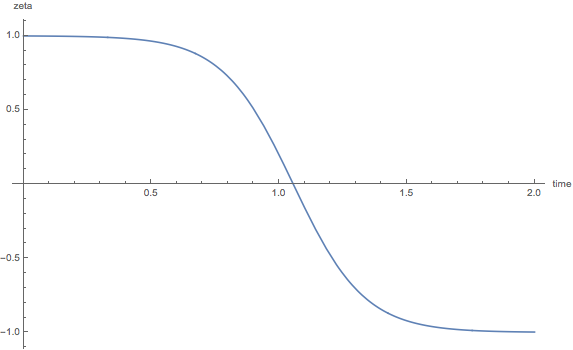
\includegraphics[width=0.5\textwidth]{Images/NeoclassicalDecay.png}
%   \caption{Non-exponential decay of $\zeta$, $\frac{g}{\kappa} = 50, \zeta(0) \approx 1$} \label{fig:neoclassical}
% \end{figure}
\subsubsection{Steady State}
We now set all derivatives to zero, and consider the asymptotic solutions to the mean-field equations, which must satisfy:
\begin{align}
  -ig \beta -i \Epsilon &= 0 \\
  ig\alpha \zeta &= 0
\end{align}
from which are obvious two branches of solutions $\rightarrow \zeta = 0$ or $\alpha = 0$. We take $\alpha = 0$ and from \cref{eq:alpha} and \cref{eq:pseudospin}
\begin{align}
  \beta &= -\frac{\Epsilon}{g} \\
  \zeta &= \mp \sqrt{1 - {\left( \frac{2\Epsilon}{g} \right)}^2}
\end{align}
Increasing drive through the critical point $\Epsilon = \frac{g}{2}$ the difference under the square root becomes negative and the inversion $\zeta$ imaginary and unphysical. We take up the other branch $\zeta = 0$, and from \cref{eq:alpha}
\begin{align}
  \beta &= \pm \frac{\alpha}{2|\alpha|} \\
  \zeta &= 0
\end{align}
with $\alpha$ a solution to
\begin{equation}
  \alpha = -i \Epsilon{\left ( \kappa \pm i \frac{g}{2|\alpha|} \right )}^{-1}
  \label{eq:alphacondnotdet}
\end{equation}

\begin{figure}[h]
  \begin{minipage}{.5\linewidth}
    \centering
    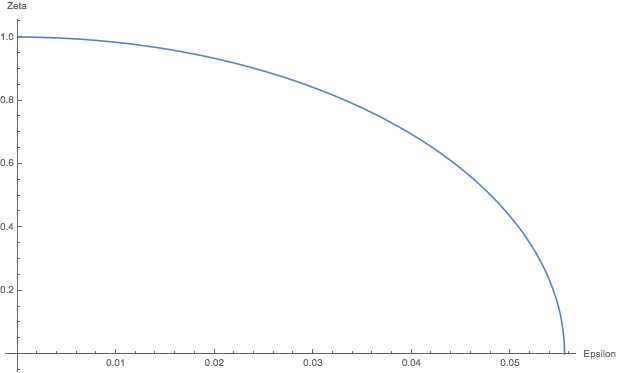
\includegraphics[width=1\textwidth]{Images/MeanFieldBelowCritical.png}
    \caption{$\zeta$ approaches zero with increasing drive strength (positive branch)}\label{fig:zeta}
  \end{minipage}%
  \begin{minipage}{.5\linewidth}
    \centering
    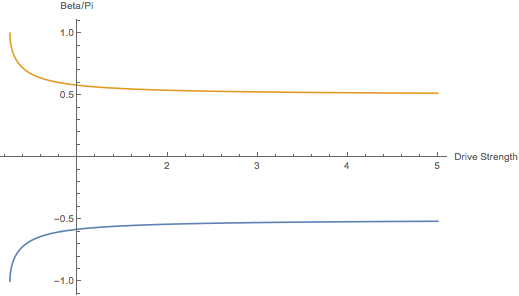
\includegraphics[width=1\textwidth]{Images/MeanFieldAboveCritical.png}
    \caption{Phase of $\beta$ with increasing drive greater than critical}\label{fig:alpha}
  \end{minipage}
  \caption{$\alpha$ and $\zeta$ as the drive strength $\Epsilon$ moves up to through and beyond the critical point}
\end{figure}

in \cref{fig:alpha} the phase bistability above the critical point is obvious. The two $\beta$ solution branches start coincident in phase ($\pi$ and $-\pi$) at drive strengths just above critical and quickly move to opposite sides of the Bloch sphere ($-\frac{\pi}{2}$ and $\frac{\pi}{2}$).

The phase of $\beta$ above the critical point follows the phase of $\alpha$, either aligned or antialigned. This spontaneous development of phase bistability Alsing and Carmichael call `Spontaneous Dressed State Polarisation' \cite{Alsing1990}. Referred to the fully quantum model, each of the two phases corresponds to a the system ascending different sets of rungs of the Jaynes Cummings ladder, either $\ket{E_{n, U}}$ or $\ket{E_{n, L}}$
\subsubsection{Non-zero detuning}
Solving \cref{eq:alpha}, \cref{eq:beta}, \cref{eq:zeta} in the steady state gives
\begin{align}
  \alpha& = i \Epsilon\frac{1}{[\kappa-i(\Delta \omega \mp sgn(\Delta \omega) \frac{g^2}{\sqrt{\Delta \omega^2 +4g^2 |\alpha|^2}})]}
\end{align}
as a condition that $\alpha$ should satisfy, and
\begin{align}
  \beta& = \pm sgn(\Delta \omega) \frac{g \alpha}{\sqrt{\Delta \omega^2 + 4 g^2 |\alpha|^2}}\\
  \zeta& = \mp \sqrt{1-4|\beta|^2}
\end{align}
for $\beta$ and $\zeta$, where $sgn(\Delta \omega)$ is the sign of the detuning with $sgn(0) = 1$.

The expression for $\alpha$ is a Lorentzian, in which is obvious a nonlinear dispersion which diverges as $|\alpha|^2 \rightarrow 0$

A surface plot of $|\alpha|^2 \approx n$ is shown in \ref{fig:MeanFieldvsQuantum}.
\subsection{Numerics}
\begin{figure*}
 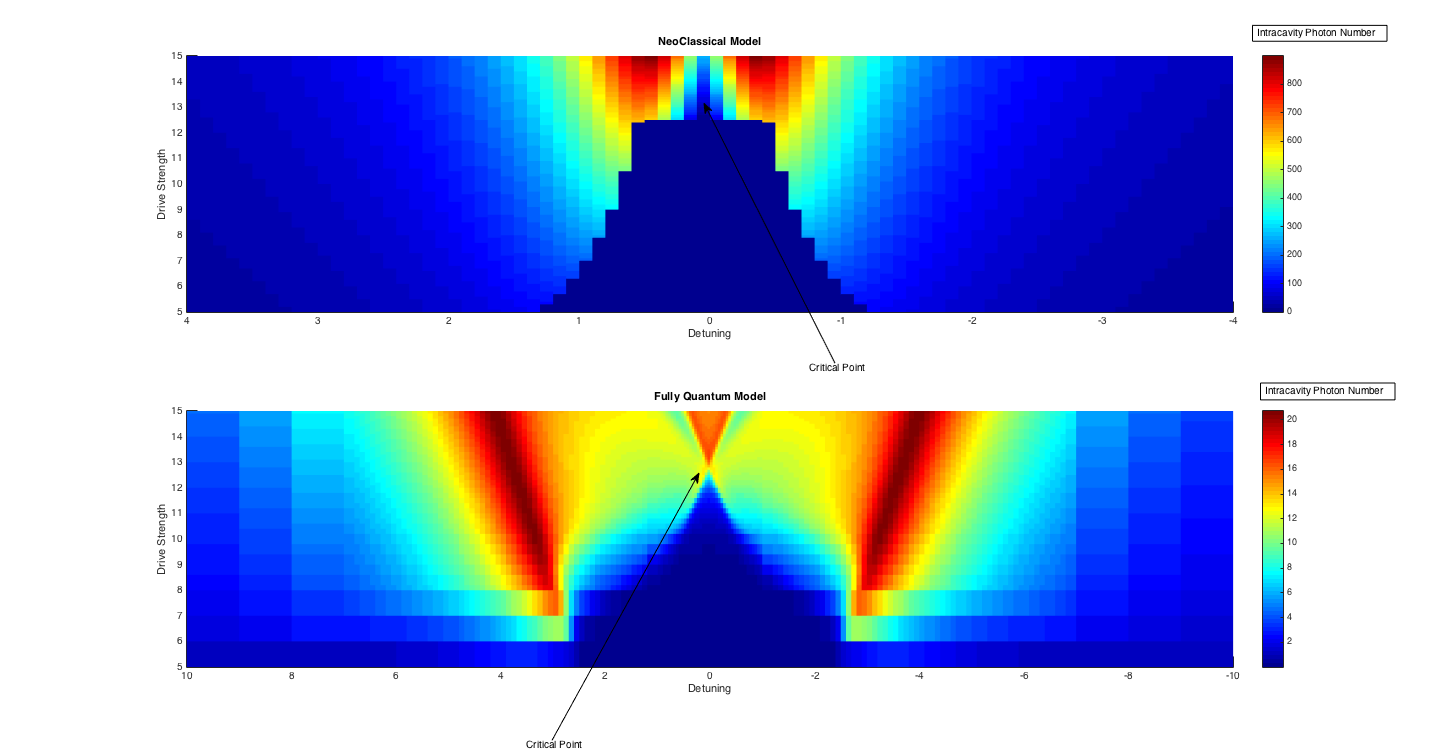
\includegraphics[width=\textwidth]{Images/MeanFieldvsQuantum.png}
 \caption{Comparison of mean field and fully quantum contour plots with critical points at $\frac{\Epsilon}{2}$ highlighted}\label{fig:MeanFieldvsQuantum}
 \end{figure*}

Truncating the master equation density matrix Fock state expansion produces a finite set of coupled differential equations for the components, from which for low photon occupation expectation values in full quantum generality can be generated to high accuracy. This method does however scale incredible poorly in the system size (the number of elements in the density matrix $\propto N^2$, where N is the dimension of the system Hilbert space. The method of quantum trajectories scales much better \cite{Molmer1993} $\propto N$ by considering the wavefunction stochastically). Setting the time derivatives to zero here yields a matrix equation, which given the positive definiteness and hermiticity conditions on the density matrix yields to a Cholesky solver \cite{Press1992}. We use the Matlab and Python solvers as exposed by QuTiP \cite{Johansson2013a} and qotoolbox\cite{Tan1999a}. For the time dependent solutions, we also use fourth order runge-kutta methods provided in both libaries.

The multiple peaks in the bilorentzian (at the bottom of \cite[Figure 1]{Carmichael2015}) as we move from large to little detuning are a mark of multiphoton blockades and their breaking through.

The sides of the Lorentzians correspond to domains of coexistence between the near vacuum state and the high occupation state \cite{Carmichael2015}, and the phase transition between the two at this boundary is of first order, its discontinuity relating to the breaking down of blockade. The transition as the drive strength moves through the critical point is of second order, as indicated in the plots of the approach to equilibrium below, where critical slowing in the approach close to the critical point reveals its nature.

All such features are obvious in our plots in \cref{fig:MeanFieldvsQuantum}, where the quantum results in \cite{Carmichael2015} have been reproduced. Computationally solving the for $\alpha$ in the meanfield condition above yields the first plot.

Numerical calculation of the Q function along the walls of the bilorentzian show a marked bimodality in amplitudeThe development of this Q function bimodality is echoed in the Wigner representation, and is clear in \cref{fig:Qbistabilities}, although the parameters are different to those in \cref{fig:MeanFieldvsQuantum} and in \cite{Carmichael2015}. Moving through the critical point in the drive, the Q function bifurcates, this time in phase, where two coexistent gaussian peaks in phase space mark the phase bistability discussed above.
\begin{figure}
 \begin{minipage}{.5\linewidth}
  \centering
  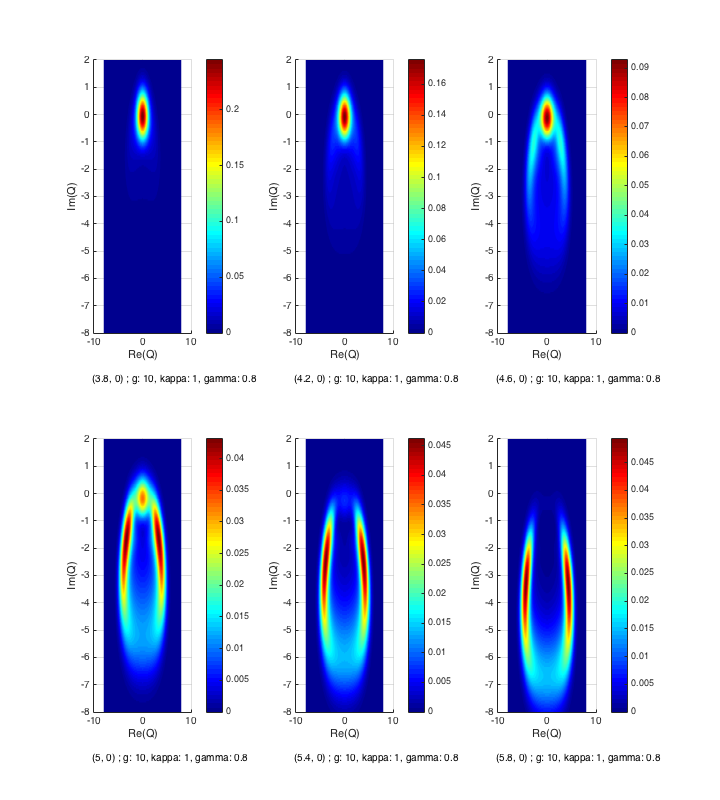
\includegraphics[width=1\textwidth]{Images/Q-Bistability-OnResonance.png}
  \caption{Development of phase bistability in the W function for fixed detuning, with drive moving through the critical point at $\frac{\Epsilon}{2}$}
  \end{minipage}%
  \begin{minipage}{.5\linewidth}
      \centering
      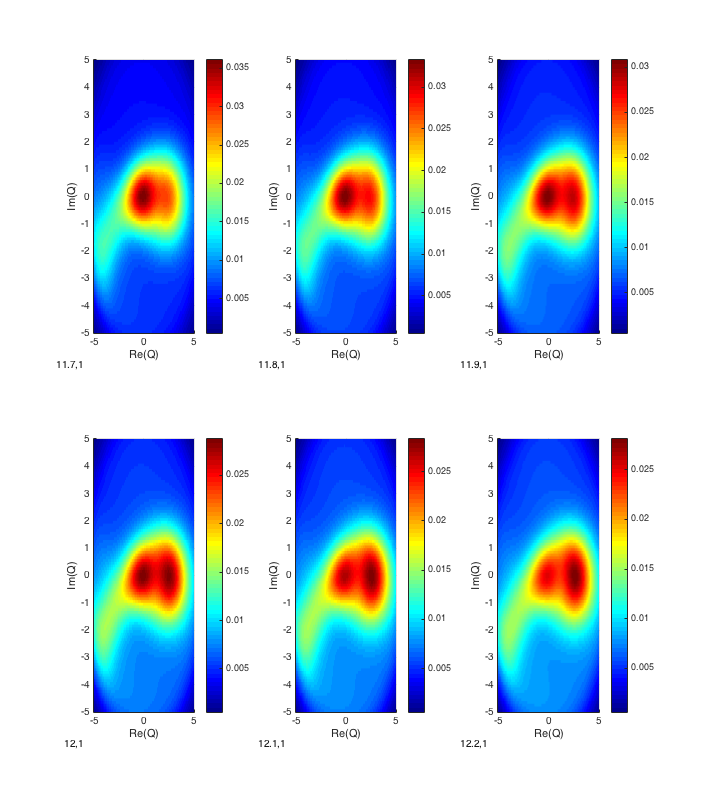
\includegraphics[width=1\textwidth]{Images/Q-Bistability.png}
      \caption{W functions with changing detuning and fixed drive. Note the probability fringes to the right connecting the peaks by spontaneous emission}
  \end{minipage}
  \caption{Q-bistabilities}\label{fig:Qbistabilities}
\end{figure}

\begin{figure*}
  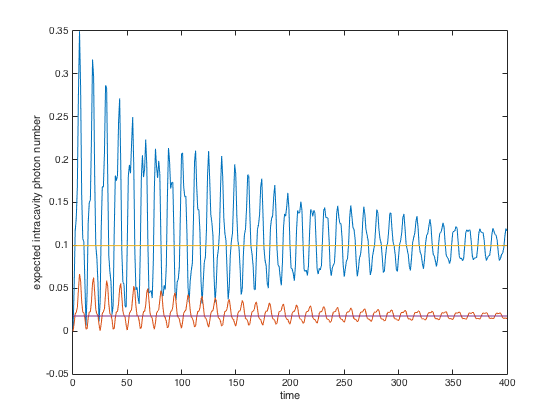
\includegraphics[width=\textwidth]{Images/CriticalSlowing.png}
  \caption{Time Dependent Solutions with g=0.5, $\kappa$ = 0.01, blue line is (0.24, 1), red line is (0.1, 1)}\label{fig:CriticalSlowing}
\end{figure*}

\subsection{Spontaneous Emission}.

We now reintroduce the spontaneous emission parameter, both in the mean-field and the quantum case. In \ref{fig:Qbistabilities} we show Q functions along the inner walls of the bilorentzian in \ref{fig:MeanFieldvsQuantum} and through the critical point in the drive, with the spontaneous emission parameter present.

Deexcitation fringes are clear in \ref{fig:Qbistabilities} where a spontaneous emission rate $ \gamma = \frac{\kappa}{2}$ connects the peaks of both of the bistabilities: in phase and in amplitude. Given the interpretation of such bimodal quasi-probability functions in the zero detuning case as as having a probability peak for the occupation of each ladder, it is clear that spontaneous emission serves to induce ladder-switching. It is this ladder switching that washes out the semiclassical bistability in the quantum regime.

We return to mean-field equations. The optical Bloch equations with spontaneous emission read:
\begin{align}
\frac{d \alpha}{dt} &= -(\kappa - i \Delta \omega)\alpha - ig \beta - i\Epsilon\label{eq:alphase}\\
\frac{d \beta}{dt} &= -(\frac{\gamma}{2}-i\Delta\omega)\beta+ig\alpha\zeta \label{eq:betase}\\
\frac{d\zeta}{dt} &= -\gamma (\zeta +1)+2ig(\alpha^*\beta-\alpha\beta^*) \label{eq:zetase}
\end{align}
In the steady state \cref{eq:alphase} becomes
\begin{align}
  \beta &= \frac{ig\alpha\zeta}{\frac{\gamma}{2}-i\Delta\omega}
\end{align}
from which in \cref{eq:zetase} in steady-state
\begin{align}
  0 &= -\gamma(\zeta+1)+2ig\frac{ig|\alpha|^2\zeta\frac{\gamma}{2}2}{\frac{\gamma^2}{4}+\Delta\omega^2} \\
  \implies \zeta &= \frac{1}{\frac{-2g^2|\alpha|^2}{\frac{\gamma^2}{4} +\Delta\omega^2}-1} \\
  &= \frac{1}{\frac{-2g^2|\alpha|^2 - \frac{\gamma^2}{4}-\Delta\omega^2}{\frac{\gamma^2}{4} +\Delta\omega^2}}
\end{align}
putting the above together yields
\begin{align}
  \beta &= \frac{ig\alpha\zeta}{\frac{\gamma}{2}-i\Delta\omega}\\
  &= \frac{ig\alpha}{\frac{(-2g^2|\alpha|^2-\frac{\gamma^2}{4}-\Delta\omega^2)(\frac{\gamma}{2}-i\Delta\omega)}{\frac{\gamma^2}{4}+\Delta\omega^2}}\\
  &= \frac{ig\alpha}{\frac{-2g^2|\alpha|^2-\frac{\gamma^2}{4}-\Delta\omega^2}{\frac{\gamma}{2}+i\Delta\omega^2}}\\
  &= \frac{ig\alpha(\frac{\gamma}{2}+i\Delta\omega)}{-2g^2|\alpha|^2-\frac{\gamma^2}{4}-\Delta\omega^2} \label{eq:betasolved}
\end{align}
\cref{eq:alphase} in the steady state with  \cref{eq:betasolved} becomes a condition for $\alpha$
\begin{align} % Here be weird bugs
0&=-(\kappa-i\Delta\omega)\alpha-ig\beta-i\Epsilon \\
0&=-{(\kappa-i\Delta\omega)}\alpha-g\frac{ig(\frac{\gamma}{2}+i\Delta\omega)}{-2g^2|\alpha|^2-\frac{\gamma^2}{4}-\Delta\omega^2}\alpha-i\Epsilon \\
\implies \alpha &= -i\Epsilon \frac{1}{\kappa-i\Delta\omega+\frac{g^2(\frac{\gamma}{2}+i\Delta\omega)}{\frac{\gamma^2}{4}+{\Delta\omega}^2+2g{|\alpha|}^2}}\label{eq:alphadetdiss}
\end{align}
Setting $\gamma$ and $\Delta\omega$ to zero, the condition becomes
\begin{equation}
  \alpha = -i\Epsilon\frac{1}{\kappa}
\end{equation}
which is notably not the same as \cref{eq:alphacondnotdet}.

\subsubsection{Difference between limits}\cite{Alsing1990}
  The presence of $\gamma$ in the Maxwell-Bloch Equations changes the asymptotic solutions, even if $\gamma$ is set to zero in these solutions. This is down to the breaking of the conservation law $4|\beta|^2 +\zeta^2 = 1$ by the presence of spontaneous emission. The solutions in the case that the limit is taken after steady state requirement is imposed are those of absorptive optical bistability. In the limit $\frac{\gamma}{\kappa} \rightarrow 0$ the rate at which these steady states becomes vanishingly small

\Cref{eq:alphadetdiss} is the classical solution for the steady state of a saturable two level transition, with a saturation photon number ($I \propto |\alpha|^2 \approx n_{sat}$) of $n_{sat} = \frac{\gamma^2}{8g^2}$.

\subsection{Dispersion}
We now move to the dispersive regime, where the cavity qubit detuning $\delta_{cq}$ is very large compared to the other frequencies in the problem. Following the work of Ginossar and Bishop \cite{Bishop2010}, we build a semiclassical model for the system
\begin{equation}
\mathscr{H} = \omega_c \cre \ann + ( \omega_c - \Delta ) \sigma_z /2 + \frac{\chi}{\sqrt{2}} (\ann + \cre ) cos(\omega_d t)
\end{equation}
which is solvable but for the term $\Delta$, defined
\begin{equation}
        \Delta = \sqrt{\delta^2 +4 g ^2 N}
\end{equation}
In which the operator $N = \cre \ann $ appears non-trivially. Rewriting the hamiltonian in terms of the generalised coordinates
\begin{equation}
        \mathscr{H} = \omega_c/1 (X^2 + P^2 + \sigma_z) + \xi X cos(\omega_d t) - \sigma_z /2 \sqrt{2g^2(X^2+P^2+\sigma_z) + \delta^2}
\end{equation}
where the $\delta$ term has been split. We make the semiclassical approximation by treating P and X as numbers, and make the claim that such an assumption holds for all N (intracavity photon number) much greater than $N_{crit}$, where $N_{crit}$ is equal to $\frac{\delta^2}{g^2}$.
From Hamilton's equations for the (semi-) classical Hamiltonian
\begin{align}
        \frac{d\mathscr{H}}{dX} &= \frac{dP}{dt}\\
        \frac{d\mathscr{H}}{dP} &= -\frac{dX}{dt}
\end{align}
in the steady state, setting the second derivatives of the quadratures X \& P to zero and solving for the amplitude $A = X^1 + P^2$, we find
\begin{equation}
        A^2 = \frac{\omega_d^2\xi}{\{\omega_d^2 - [\omega_c - \chi (A) ]^2 \}^2+ \kappa^2 \omega_d^2}
\end{equation}
where
\begin{equation}
        \chi(A) = \sigma_z \frac{g^2}{\sqrt{2g^2(A^2 + \sigma_z) + \delta^2}}
\end{equation}
inverting the equation and solving for $\xi$ as a function of $A^2$, we retrieve for the amplitude as a function of the detuning and the drive strength:
\begin{figure*}
        \includegraphics[width=\textwidth]{Images/SemiclassicalBistability.png}
        \caption{Semiclassical Amplitude as a function of drive and detuning}
\end{figure*}
Areas where the amplitude is not 1-1 (for given drive) indicate the existence of bistability, where the negative gradient intermediate state is metastable, and the system is stable along the upper and lower curves. These regions in the quantum case are washed out by switching induced by quantum fluctuations, and the amplitude in the quantum case can be qualitatively expected to 'average out' the bistability and lie between the two stable states on this plot. Indeed, this effect is visible in the next plot. We see more interesting features here too, most notably a dip in the quantum amplitude, where there is destructive interference between the two stable paths. In a sense, the quantum amplitude is characterised by the switching rate, where at a given detuning, the upwards switching drags the curve upwards and the downwards downwards.


\printbibliography\
\end{document}
